\documentclass[aspectratio=169,utf8,t]{beamer}

% Idioma e Codificacao
\usepackage[brazilian]{babel}
\usepackage{booktabs}
\usepackage{array}
\usepackage{listings}

% Carrega o Tema Modelo dos Scouts (Widescreen 16:9, Nunito Sans)
\usetheme{scouts}

% Configuracao para Codigo-Fonte (SQL / JSON / Python)
\lstset{
    basicstyle=\ttfamily\scriptsize,
    keywordstyle=\bfseries\color{ScoutNavy},
    stringstyle=\color{ScoutGreen},
    commentstyle=\itshape\color{gray},
    backgroundcolor=\color{black!3},
    frame=single,
    rulecolor=\color{black!15},
    breaklines=true,
    showstringspaces=false,
    tabsize=2
}

% Metadados Institucionais
\author{Prof. Me. Reginaldo Fernandes}
\institute{Instituto Federal do Ceará -- Campus Tauá \\ Tecnologia em Análise e Desenvolvimento de Sistemas}
\title{Bancos de Dados Não-Relacionais}
\subtitle{Aula 01: O Paradigma Pós-Relacional \& Diretrizes da Disciplina}
\date{29 de Setembro de 2026}

\begin{document}

% ------------------------------------------------------------------------------
% Capa da Apresentacao
% ------------------------------------------------------------------------------
\changecolours[inverse]{ScoutGreen}
\frame[plain]{\titlepage}

% ------------------------------------------------------------------------------
% Sumario Executivo da Aula
% ------------------------------------------------------------------------------
\changecolours{ScoutGreen}
\begin{frame}{Agenda do Encontro}
  \vspace{0.4cm}
  \tableofcontents
\end{frame}

% ------------------------------------------------------------------------------
% Modulos da Aula
% ------------------------------------------------------------------------------
\changecolours{ScoutGreen}
\section{Diretrizes \& Avaliação}

% ------------------------------------------------------------------------------
\twocolframe[title={Visão Geral da Disciplina: ADS16},leftcol=7cm,rightcol=7cm]{%
  \alert{Estrutura do Curso}\par
  \itemseps[topsepi=2mm,itemsepi=3mm,labelsep=2mm,leftmargini=4mm]
  \begin{itemize}
    \item \textbf{Carga Horária:} 40 horas no semestre.
    \item \textbf{Total de Encontros:} 20 encontros (2h/aula cada).
    \item \textbf{Horário Regular:} Terças-feiras.
    \item \textbf{Ambiente:} Laboratório de Informática.
    \item \textbf{Metodologia:} Aulas teórico-práticas com programação.
  \end{itemize}
}{%
  \alert{Pilares de Aprendizagem}\par
  \itemseps[topsepi=2mm,itemsepi=3mm,labelsep=2mm,leftmargini=4mm]
  \begin{itemize}
    \item \textbf{Ambiente Docker:} Orquestração rápida de Redis, MongoDB e Neo4j.
    \item \textbf{Engenharia de Dados:} Alta escala, concorrência e particionamento.
    \item \textbf{Modernização:} Introdução a Bancos Vetoriais para Inteligência Artificial.
  \end{itemize}
}

% ------------------------------------------------------------------------------
\begin{frame}{Sistema de Avaliação da Disciplina}
  \vspace{-0.2cm}
  \begin{center}
    {\normalsize \textbf{Fórmula Regimental de Média por Período (N1 e N2):}}\par
    \vspace{0.15cm}
    {\large \alert{$\mathbf{\text{Nota} = (\text{AVT} \times 0{,}40) + (\text{AVP} \times 0{,}40) + (\text{Listas} \times 0{,}20)}$}}
  \end{center}

  \vspace{0.2cm}

  \begin{columns}[t]
    \begin{column}{0.48\textwidth}
      \footnotesize
      \alert{AVT (40\%) -- Avaliação Teórica}
      \begin{itemize}
        \item Prova individual sem consulta.
        \item Fundamentos, CAP/PACELC, ACID vs BASE e arquitetura.
      \end{itemize}
      \vspace{0.2cm}
      \alert{AVP (40\%) -- Avaliação Prática}
      \begin{itemize}
        \item \textbf{AVP1 (N1):} Desafio prático individual em laboratório.
        \item \textbf{AVP2 (N2):} Projeto prático integrado em \textbf{duplas}.
      \end{itemize}
    \end{column}

    \begin{column}{0.48\textwidth}
      \footnotesize
      \alert{Listas (20\%) -- Avaliação Contínua}
      \begin{itemize}
        \item Exercícios práticos de laboratório e fixação.
        \item Entrega até a data da avaliação teórica do período.
      \end{itemize}
      \vspace{0.2cm}
      \alert{Avaliação Final (AF)}
      \begin{itemize}
        \item Prova final de recuperação ao término do semestre.
      \end{itemize}
    \end{column}
  \end{columns}
\end{frame}

% ------------------------------------------------------------------------------
\twocolframe[title={Diretriz dos Sábados Letivos},leftcol=7cm,rightcol=7cm]{%
  \alert{10/10/2026 -- Sábado Letivo 01}\par
  \itemseps[topsepi=2mm,itemsepi=3mm,labelsep=2mm,leftmargini=4mm]
  \begin{itemize}
    \item \textbf{Dia Sem Conteúdo Novo.}
    \item \textbf{Oficina Prática de Ferramentas:} Orquestração de containers com Docker Compose.
    \item Subida e teste de instâncias de Redis e MongoDB.
    \item Resolução orientada da Lista Preparatória 1.
  \end{itemize}
}{%
  \alert{14/11/2026 -- Sábado Letivo 02}\par
  \itemseps[topsepi=2mm,itemsepi=3mm,labelsep=2mm,leftmargini=4mm]
  \begin{itemize}
    \item \textbf{Dia Sem Conteúdo Novo.}
    \item \textbf{Laboratório de Fixação:} Simulado e revisão prática integrada (Redis + MongoDB).
    \item Plantão de dúvidas antes de AVP1 (17/11) e AVT1 (24/11).
    \item Fechamento da Lista de Exercícios 1.
  \end{itemize}
}

\changecolours{ScoutNavy}
\section{Contexto Histórico \& Big Data}

% ------------------------------------------------------------------------------
\twocolframe[title={O Domínio do Modelo Relacional (1970 -- 2000)},leftcol=7cm,rightcol=7cm]{%
  \alert{A Era Codd e a Álgebra Relacional}\par
  \itemseps[topsepi=2mm,itemsepi=3mm,labelsep=2mm,leftmargini=4mm]
  \begin{itemize}
    \item Proposto por Edgar F. Codd em 1970 (IBM).
    \item Base matemática na álgebra relacional e conjuntos.
    \item Tabelas rígidas com chaves primárias e integridade.
    \item \textbf{Premissa Central:} Modelo desenhado para operar em \textbf{um único servidor centralizado}.
  \end{itemize}
}{%
  \alert{Garantias Transacionais ACID}\par
  \itemseps[topsepi=2mm,itemsepi=2.5mm,labelsep=2mm,leftmargini=4mm]
  \begin{itemize}
    \item \textbf{A}tomicidade: Tudo ou nada na transação.
    \item \textbf{C}onsistência: Regras e restrições sempre válidas.
    \item \textbf{I}solamento: Concorrência sem interferência.
    \item \textbf{D}urabilidade: Persistência garantida em disco.
    \item \textbf{Sucesso:} Eliminou inconsistências por 30 anos.
  \end{itemize}
}

% ------------------------------------------------------------------------------
\twocolframe[title={O Ponto de Inflexão: A Web 2.0 e os 3 Vs},leftcol=7cm,rightcol=7cm]{%
  \alert{Volume \& Velocidade}\par
  \itemseps[topsepi=2mm,itemsepi=3mm,labelsep=2mm,leftmargini=4mm]
  \begin{itemize}
    \item \textbf{Volume:} Salto de gigabytes para terabytes e petabytes diários gerados por bilhões de usuários.
    \item Volume total excede o hardware de uma única máquina.
    \item \textbf{Velocidade:} Milhões de requisições por segundo.
    \item Exigência de tempo de resposta em milissegundos.
  \end{itemize}
}{%
  \alert{Variedade}\par
  \itemseps[topsepi=2mm,itemsepi=3mm,labelsep=2mm,leftmargini=4mm]
  \begin{itemize}
    \item Dados heterogêneos: JSON, logs, redes e sensores IoT.
    \item Esquemas que mudam diariamente sem possibilidade de paradas programadas para migração (\texttt{ALTER TABLE}).
  \end{itemize}
}

\changecolours{ScoutBlue}
\section{Gargalos do Relacional}

% -------------------------------------------------------------
% TOPICO 1 - SLIDE A: TEORIA E CUSTOS DE ESCALA
% -------------------------------------------------------------
\twocolframe[title={Escala Vertical vs. Escala Horizontal: Análise},leftcol=7cm,rightcol=7cm]{%
  \alert{Escala Vertical (Scale-Up -- RDBMS)}\par
  \itemseps[topsepi=2mm,itemsepi=3mm,labelsep=2mm,leftmargini=4mm]
  \begin{itemize}
    \item \textbf{Abordagem Clássica:} Adicionar mais CPUs, memória RAM e SSDs mais rápidos ao mesmo servidor.
    \item \textbf{Custo Exponencial:} Duplicar a capacidade pode multiplicar o preço do hardware por 10 vezes.
    \item \textbf{Teto Físico:} Limite de barramento da placa-mãe e arquitetura de processador.
    \item \textbf{Ponto Único de Falha (SPOF):} Queda da máquina derruba toda a aplicação.
  \end{itemize}
}{%
  \alert{Escala Horizontal (Scale-Out -- NoSQL)}\par
  \itemseps[topsepi=2mm,itemsepi=3mm,labelsep=2mm,leftmargini=4mm]
  \begin{itemize}
    \item \textbf{Abordagem Nativa:} Adicionar múltiplos servidores comuns em cluster (\textit{commodity hardware}).
    \item \textbf{Custo Linear:} Expansão elástica e gradual conforme a demanda real de tráfego.
    \item \textbf{Alta Resiliência:} Tolerância nativa a falhas com réplicas automáticas de dados.
    \item \textbf{Expansão Ilimitada:} Cluster cresce de 3 para centenas de nós sem interrupções.
  \end{itemize}
}

% -------------------------------------------------------------
% TOPICO 1 - SLIDE B: DIAGRAMA EM TELA CHEIA
% -------------------------------------------------------------
\begin{frame}{Topologia: Servidor Único vs. Cluster Distribuído}
  \vspace{-0.3cm}
  \makebox[\linewidth][c]{%
    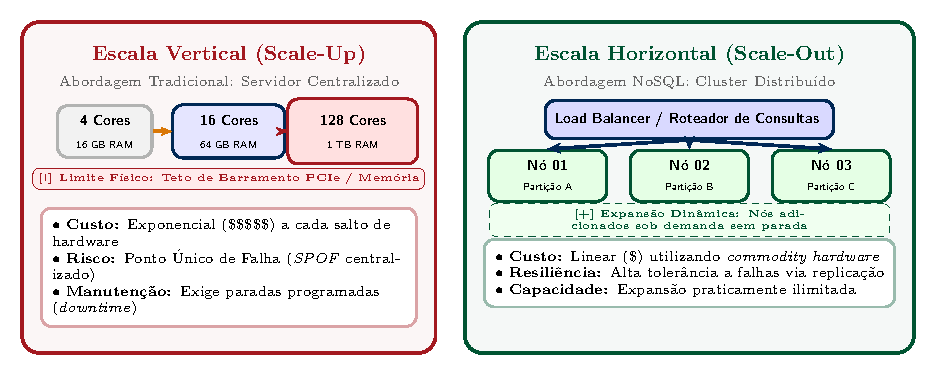
\includegraphics[width=13.2cm,height=4.8cm,keepaspectratio]{figuras/fig_escala.pdf}%
  }\par
  \vspace{0.15cm}
  \centering
  {\footnotesize \textbf{Takeaway:} \textcolor{ScoutBlue}{Enquanto o Scale-Up encontra barreiras físicas e financeiras, o Scale-Out viabiliza crescimento elástico.}}
\end{frame}

% -------------------------------------------------------------
% TOPICO 2 - SLIDE A: O PROBLEMA DOS JOINS DISTRIBUIDOS
% -------------------------------------------------------------
\twocolframe[title={O Gargalo dos JOINs em Clusters},leftcol=7cm,rightcol=7cm]{%
  \alert{Execução Local em Servidor Único}\par
  \itemseps[topsepi=2mm,itemsepi=3mm,labelsep=2mm,leftmargini=4mm]
  \begin{itemize}
    \item O motor SQL resolve o \texttt{JOIN} buscando ponteiros diretos em memória RAM ou bloco de SSD local.
    \item Operação extremamente rápida com latência inferior a 1 milissegundo.
    \item O algoritmo de junção se beneficia de índices em memória e do cache local de páginas (\textit{buffer pool}).
  \end{itemize}
}{%
  \alert{O Fenômeno do Network Shuffle}\par
  \itemseps[topsepi=2mm,itemsepi=3mm,labelsep=2mm,leftmargini=4mm]
  \begin{itemize}
    \item Em um cluster particionado, as tabelas residem em servidores físicos distintos da rede.
    \item Realizar o cruzamento obriga os nós a serializar e transmitir milhões de tuplas pelos cabos e switches.
    \item \textbf{Impacto Severo:} O tráfego massivo satura a rede e faz a latência saltar de milissegundos para dezenas de segundos!
  \end{itemize}
}

% -------------------------------------------------------------
% TOPICO 2 - SLIDE B: DIAGRAMA EM TELA CHEIA
% -------------------------------------------------------------
\begin{frame}{Anatomia do Network Shuffle: Saturação de Rede}
  \vspace{-0.3cm}
  \makebox[\linewidth][c]{%
    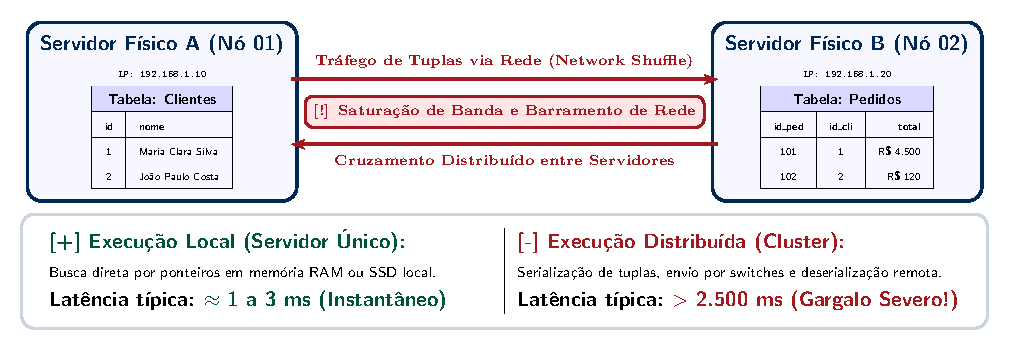
\includegraphics[width=13.2cm,height=4.8cm,keepaspectratio]{figuras/fig_gargalo_joins.pdf}%
  }\par
  \vspace{0.15cm}
  \centering
  {\footnotesize \textbf{Takeaway:} \textcolor{ScoutRed}{Cruzar dados entre servidores físicos distintos transforma a rede no gargalo principal do sistema.}}
\end{frame}

% -------------------------------------------------------------
% TOPICO 3 - SLIDE A: O DESCASAMENTO DE IMPEDANCIA
% -------------------------------------------------------------
\twocolframe[title={Descasamento de Impedância Objeto-Relacional},leftcol=7cm,rightcol=7cm]{%
  \alert{O Paradigma da Aplicação (OOP)}\par
  \itemseps[topsepi=2mm,itemsepi=3mm,labelsep=2mm,leftmargini=4mm]
  \begin{itemize}
    \item A linguagem (Python, Java) trabalha com grafos ricos de objetos em memória.
    \item Uma entidade de negócio como \texttt{Cliente} contém atributos simples, endereços aninhados e listas de pedidos.
    \item Os dados estão naturalmente agrupados para o consumo da lógica de negócio.
  \end{itemize}
}{%
  \alert{O Atrito do RDBMS \& ORM}\par
  \itemseps[topsepi=2mm,itemsepi=3mm,labelsep=2mm,leftmargini=4mm]
  \begin{itemize}
    \item A teoria relacional exige normalização estrita (3NF), forçando o fatiamento da entidade em 4 ou mais tabelas.
    \item O mapeador (ORM) adiciona sobrecarga de conversão e problemas como consultas $N+1$.
    \item \textbf{Solução em Documentos:} O formato BSON/JSON do MongoDB armazena o objeto íntegro, lido em 1 único I/O atômico!
  \end{itemize}
}

% -------------------------------------------------------------
% TOPICO 3 - SLIDE B: DIAGRAMA EM TELA CHEIA
% -------------------------------------------------------------
\begin{frame}{Mapeamento Estrutural: 3NF vs. Documento BSON Nativo}
  \vspace{-0.3cm}
  \makebox[\linewidth][c]{%
    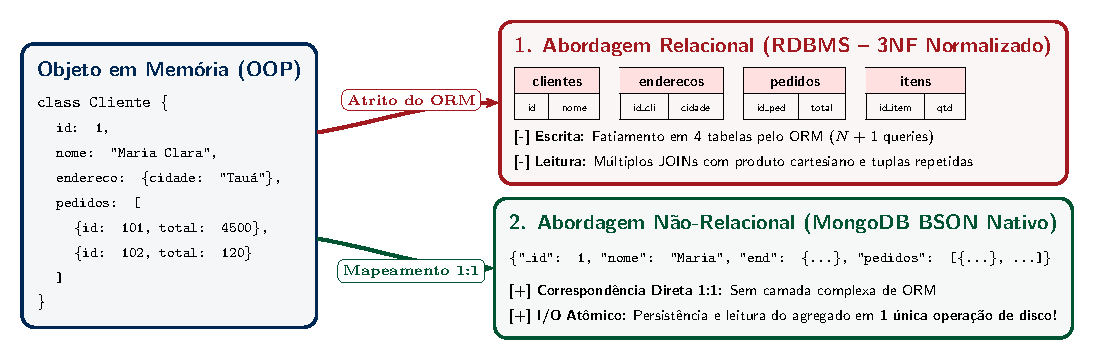
\includegraphics[width=13.2cm,height=4.8cm,keepaspectratio]{figuras/fig_impedance_mismatch.pdf}%
  }\par
  \vspace{0.15cm}
  \centering
  {\footnotesize \textbf{Takeaway:} \textcolor{ScoutGreen}{Bancos de documentos alinham a persistência física à estrutura de objetos da aplicação sem camadas de atrito.}}
\end{frame}

\changecolours{ScoutPurple}
\section{O Movimento NoSQL \& Modelos}

% ------------------------------------------------------------------------------
\twocolframe[title={O Conceito: \textit{Not Only SQL}},leftcol=7cm,rightcol=7cm]{%
  \alert{Origem e Filosofia}\par
  \itemseps[topsepi=2mm,itemsepi=3mm,labelsep=2mm,leftmargini=4mm]
  \begin{itemize}
    \item Movimento consolidado em 2009 em São Francisco.
    \item Não significa rejeitar o SQL, mas sim \textbf{\textit{Not Only SQL}} (Não Apenas SQL).
    \item \textbf{Premissa Fundamental:} Nem todos os dados do mundo se comportam como tabelas relacionais estritas.
    \item Foco em escalabilidade horizontal nativa, esquemas flexíveis (\textit{schemaless}) e alta disponibilidade.
  \end{itemize}
}{%
  \alert{Persistência Poliglota}\par
  \itemseps[topsepi=2mm,itemsepi=3mm,labelsep=2mm,leftmargini=4mm]
  \begin{itemize}
    \item Sistemas modernos utilizam bancos relacionais e NoSQL juntos.
    \item Escolhe-se a tecnologia mais adequada para cada domínio.
    \item \textbf{Exemplo:} PostgreSQL (pagamentos) + Redis (cache de sessões) + MongoDB (catálogo flexível).
  \end{itemize}
}

% ------------------------------------------------------------------------------
\twocolframe[title={Modelos NoSQL: Chave-Valor \& Documentos},leftcol=7cm,rightcol=7cm]{%
  \alert{1. Chave-Valor (Key-Value)}\par
  \itemseps[topsepi=2mm,itemsepi=2.5mm,labelsep=2mm,leftmargini=4mm]
  \textbf{Exemplos:} Redis, DynamoDB, Memcached.
  \begin{itemize}
    \item Mapeamento direto \texttt{chave} $\rightarrow$ \texttt{valor} em memória.
    \item Altíssima taxa de IOPS e latência sub-milissegundo.
    \item \textbf{Casos de Uso:} Cache acelerador, controle de sessão de login e contadores em tempo real.
  \end{itemize}
}{%
  \alert{2. Documentos (Document Store)}\par
  \itemseps[topsepi=2mm,itemsepi=2.5mm,labelsep=2mm,leftmargini=4mm]
  \textbf{Exemplos:} MongoDB, Couchbase, Firestore.
  \begin{itemize}
    \item Dados armazenados em documentos JSON/BSON aninhados.
    \item Suporte nativo a arrays, objetos embutidos e índices.
    \item \textbf{Casos de Uso:} Catálogos de e-commerce, perfis de usuários e cadastros com esquema evolutivo.
  \end{itemize}
}

% ------------------------------------------------------------------------------
\twocolframe[title={Modelos NoSQL: Colunas \& Grafos},leftcol=7cm,rightcol=7cm]{%
  \alert{3. Família de Colunas (Wide-Column)}\par
  \itemseps[topsepi=2mm,itemsepi=2.5mm,labelsep=2mm,leftmargini=4mm]
  \textbf{Exemplos:} Apache Cassandra, ScyllaDB, HBase.
  \begin{itemize}
    \item Linhas com colunas dinâmicas em anel distribuído.
    \item Otimizado para altíssimo volume de gravação contínua.
    \item \textbf{Casos de Uso:} Telemetria IoT, séries temporais, métricas de monitoramento e logs analíticos.
  \end{itemize}
}{%
  \alert{4. Grafos (Graph Database)}\par
  \itemseps[topsepi=2mm,itemsepi=2.5mm,labelsep=2mm,leftmargini=4mm]
  \textbf{Exemplos:} Neo4j, Amazon Neptune, ArangoDB.
  \begin{itemize}
    \item Vértices (nós), arestas (relacionamentos) e propriedades.
    \item Travessia direta de ponteiros sem múltiplos JOINs.
    \item \textbf{Casos de Uso:} Redes sociais, motores de recomendação e detecção de fraudes financeiras.
  \end{itemize}
}

% ------------------------------------------------------------------------------
\twocolframe[title={Bancos Vetoriais \& IA (Modernização)},leftcol=7cm,rightcol=7cm]{%
  \alert{Vector Databases na Era da IA}\par
  \itemseps[topsepi=2mm,itemsepi=3mm,labelsep=2mm,leftmargini=4mm]
  \begin{itemize}
    \item Dados não estruturados convertidos em vetores matemáticos multidimensionais (\textbf{\textit{embeddings}}).
    \item Busca por \textbf{proximidade semântica} (similaridade por cosseno), não por correspondência de texto exato.
    \item \textbf{Exemplos:} ChromaDB, Pinecone, Qdrant, Milvus.
  \end{itemize}
}{%
  \alert{Aplicações Críticas: RAG}\par
  \itemseps[topsepi=2mm,itemsepi=3mm,labelsep=2mm,leftmargini=4mm]
  \begin{itemize}
    \item \textbf{RAG (Retrieval-Augmented Generation):} Recuperação semântica para abastecer Modelos de Linguagem (LLMs).
    \item \textbf{Tópico Modernizado:} Nossa disciplina contará com uma aula prática dedicada (Aula 16) sobre este modelo!
  \end{itemize}
}

\changecolours{ScoutTeal}
\section{Prática \& Conclusão}

% ------------------------------------------------------------------------------
\begin{frame}[fragile]{Demonstração Prática: JSON vs 4 Tabelas Relacionais}
  \vspace{-0.2cm}
  \begin{columns}[t]
    \begin{column}{0.48\textwidth}
      \alert{Relacional: 4 Tabelas + 3 JOINs}\par
      \begin{lstlisting}[language=SQL]
SELECT c.nome, e.cidade, p.id_pedido, 
       i.produto, i.quantidade
FROM clientes c
JOIN enderecos e ON c.id = e.id_cliente
JOIN pedidos p ON c.id = p.id_cliente
JOIN itens_pedido i 
  ON p.id_pedido = i.id_pedido
WHERE c.id = 1;
      \end{lstlisting}
      \scriptsize Exige remontar objetos a partir de múltiplas linhas tabulares com redundâncias.
    \end{column}

    \begin{column}{0.48\textwidth}
      \alert{NoSQL: Documento Agregado}\par
      \begin{lstlisting}
{
  "_id": 1,
  "nome": "Maria Clara Silva",
  "endereco": {"cidade": "Taua", "uf": "CE"},
  "pedidos": [
    {
      "id_pedido": "PED-001",
      "itens": [
        {"produto": "Notebook", "qtd": 1}
      ]
    }
  ]
}
      \end{lstlisting}
      \scriptsize Leitura e escrita direta em 1 único I/O atômico de disco.
    \end{column}
  \end{columns}
\end{frame}

% ------------------------------------------------------------------------------
\begin{frame}{Matriz Comparativa: Relacional vs NoSQL}
  \vspace{-0.1cm}
  \resizebox{\textwidth}{!}{%
  \begin{tabular}{>{\raggedright\arraybackslash}p{3.5cm} >{\raggedright\arraybackslash}p{5.8cm} >{\raggedright\arraybackslash}p{6.0cm}}
    \toprule
    \textbf{Dimensão} & \textbf{Relacional (RDBMS)} & \textbf{Não-Relacional (NoSQL)} \\
    \midrule
    \textbf{Estrutura} & Esquema rígido e normalizado & Esquema dinâmico e flexível (\textit{schemaless}) \\
    \textbf{Escalabilidade} & Predominantemente Vertical (\textit{Scale-Up}) & Horizontal nativa em cluster (\textit{Scale-Out}) \\
    \textbf{Consistência} & Imediata e estrita (ACID) & Eventual ajustável (BASE / CAP) \\
    \textbf{Relacionamentos} & Otimizado para \texttt{JOIN}s locais & Desnormalização ou Grafos dedicados \\
    \textbf{Cenário Ideal} & Sistemas bancários, ERPs, sistemas financeiros & E-commerce, telemetria IoT, Big Data, IA / RAG \\
    \bottomrule
  \end{tabular}%
  }
\end{frame}

% ------------------------------------------------------------------------------
\twocolframe[title={Próximos Passos \& Atividades},leftcol=7cm,rightcol=7cm]{%
  \alert{Próximo Encontro: 06/10/2026}\par
  \itemseps[topsepi=2mm,itemsepi=3mm,labelsep=2mm,leftmargini=4mm]
  \textbf{Aula 02 -- Teorema CAP e BASE}
  \begin{itemize}
    \item O Teorema CAP de Eric Brewer detalhado.
    \item Teorema PACELC: a troca entre consistência e latência.
    \item Comparação formal: ACID vs BASE.
  \end{itemize}
}{%
  \alert{Tarefas do Estudante}\par
  \itemseps[topsepi=2mm,itemsepi=3mm,labelsep=2mm,leftmargini=4mm]
  \begin{itemize}
    \item Executar o script didático de apoio:
      \texttt{codigo/demonstracao\_aula01.py}.
    \item Iniciar os exercícios do Bloco 1 da \textbf{Lista de Exercícios 1 (AV3)}.
    \item Instalar o Docker para a oficina do primeiro sábado letivo (10/10).
  \end{itemize}
}


% ------------------------------------------------------------------------------
% Encerramento
% ------------------------------------------------------------------------------
\changecolours[inverse]{ScoutGreen}
\begin{frame}[plain]
  \vspace{2cm}
  \centering
  {\Huge \textbf{Dúvidas \& Discussão}}\par
  \vspace{0.8cm}
  {\large IFCE Campus Tauá -- ADS16}\par
  \vspace{0.3cm}
  {\small reginaldo.fernandes@ifce.edu.br}
\end{frame}

\end{document}
